% chap5_crowdsourcing.tex
%

\mychapter{Crowdsourcing for Real-time Question Answering}
\label{chapter:crowdsourcing}

\noindent

\section{Problem}
\label{section:crowdsourcing:problem}

Despite the progress in automatic question answering, existing systems are still far from being able to handle every human question.
For example, the winning system in TREC LiveQA 2015 shared task were able to return a good or excellent answer to less than 40\% of the questions.
And overall, according to the TREC LiveQA 2015 assessor scores, for 12.6\% of the questions none of the 21 participating systems produced even moderately useful answer, and for 30\% a good or better response.
This can happens for multiple different reasons, \eg a question is ill formulated, available data sources does not contain any relevant information, a system fails to retrieve or rank good answer candidates, \etc
As conversational agents become more popular, QA systems are increasingly expected to handle such complex questions, and to do so in (nearly) real-time, as the searcher is unlikely to wait longer than a minute or two for an answer.

One way to overcome the above mentioned challenges in complex question answering is to develop a hybrid human-computer question answering system, which could consult a crowd of workers in order to generate a good response to the user question.
This section provides some preliminary results and proposed research in crowdsourcing for real-time question answering.
Part of the described results was published at Human-Computer Question Answering workshop at NAACL 2016 conference~\cite{savenkov_crowdsourcing2016a}, and another will appear as a full paper titled ``CRQA: Crowd-powered Real-time Automated Question Answering System'' on HCOMP 2016 conference~\cite{savenkov_crqa2016}.

\section{Approach}
\label{section:crowdsourcing:approach}

In this section I explore two ways crowdsourcing can assist a question answering system that operates in (near) real-time: by providing answer {\em validation}, which could be used to filter or re-rank the candidate answers, and by {\em creating} the answer candidates directly.
First, we study if crowd workers can quickly and reliably judge the quality of the proposed answer candidates, and if it is possible to obtain reasonable written answers from the crowd within a limited amount of time.
Then, we present CRQA, a crowd-powered, near real-time automated question answering system for complex informational tasks, that incorporates a crowdsourcing module for augmenting and validating the candidate answers.
The crowd input, obtained in real-time, is integrated into CRQA via a learning-to-rank model, to select the final system answer.
Our large-scale experiments, performed on a live stream of real users questions, show that even within a one minute time limit, CRQA can produce answers of high quality.

More specifically, in this section we answer the following questions:
\begin{enumerate}
\item Can crowdsourcing be used to judge the quality of answers to non-factoid questions under a time limit?
\item Is it possible to use crowdsourcing to collect answers to real user questions under a time limit?
\item How does the quality of crowdsourced answers to non-factoid questions compare to original CQA answers, and to automatic answers from TREC LiveQA systems?
\item Can crowdsourcing be used to improve the performance of a near real-time automated question answering system?
\item What is the relative contribution of candidate answer ratings and answers provided by the workers to the overall question answering performance?
\item What are the tradeoffs in performance, cost, and scalability of using crowdsourcing for real-time question answering?
\end{enumerate}

To answer the first three questions, we conducted a series of crowdsourcing experiments using the Amazon Mechanical Turk platform\footnote{http://mturk.com}.
We used questions from the TREC LiveQA 2015 shared task, along with the system answers, rated by the NIST assessors\footnote{https://sites.google.com/site/trecliveqa2016/liveqa-qrels-2015}.
The questions for the task were selected by the organizers from the live stream of questions posted to the Yahoo! Answers CQA platform on the day of the challenge (August 31, 2015).
For these questions we also crawled their community answers, that were eventually posted on Yahoo! Answers\footnote{As the answer we took the top question, which was selected as the ``Best answer'' by the author of the question or by the community.}.

\subsection{Crowdsourcing for time-constraint answer generation and validation}
\label{section:crowdsourcing:approach:experiments}

To check if crowdsourcing can be used to judge the quality of answers under a time limit, we asked workers to rate answers to a sample of 100 questions using the official TREC rating scale:
\begin{enumerate}
\item Bad - contains no useful information
\item Fair - marginally useful information
\item Good - partially answers the question
\item Excellent - fully answers the question
\end{enumerate}

\begin{figure*}
\centering
\begin{subfigure}[b]{0.49\textwidth}
\centering
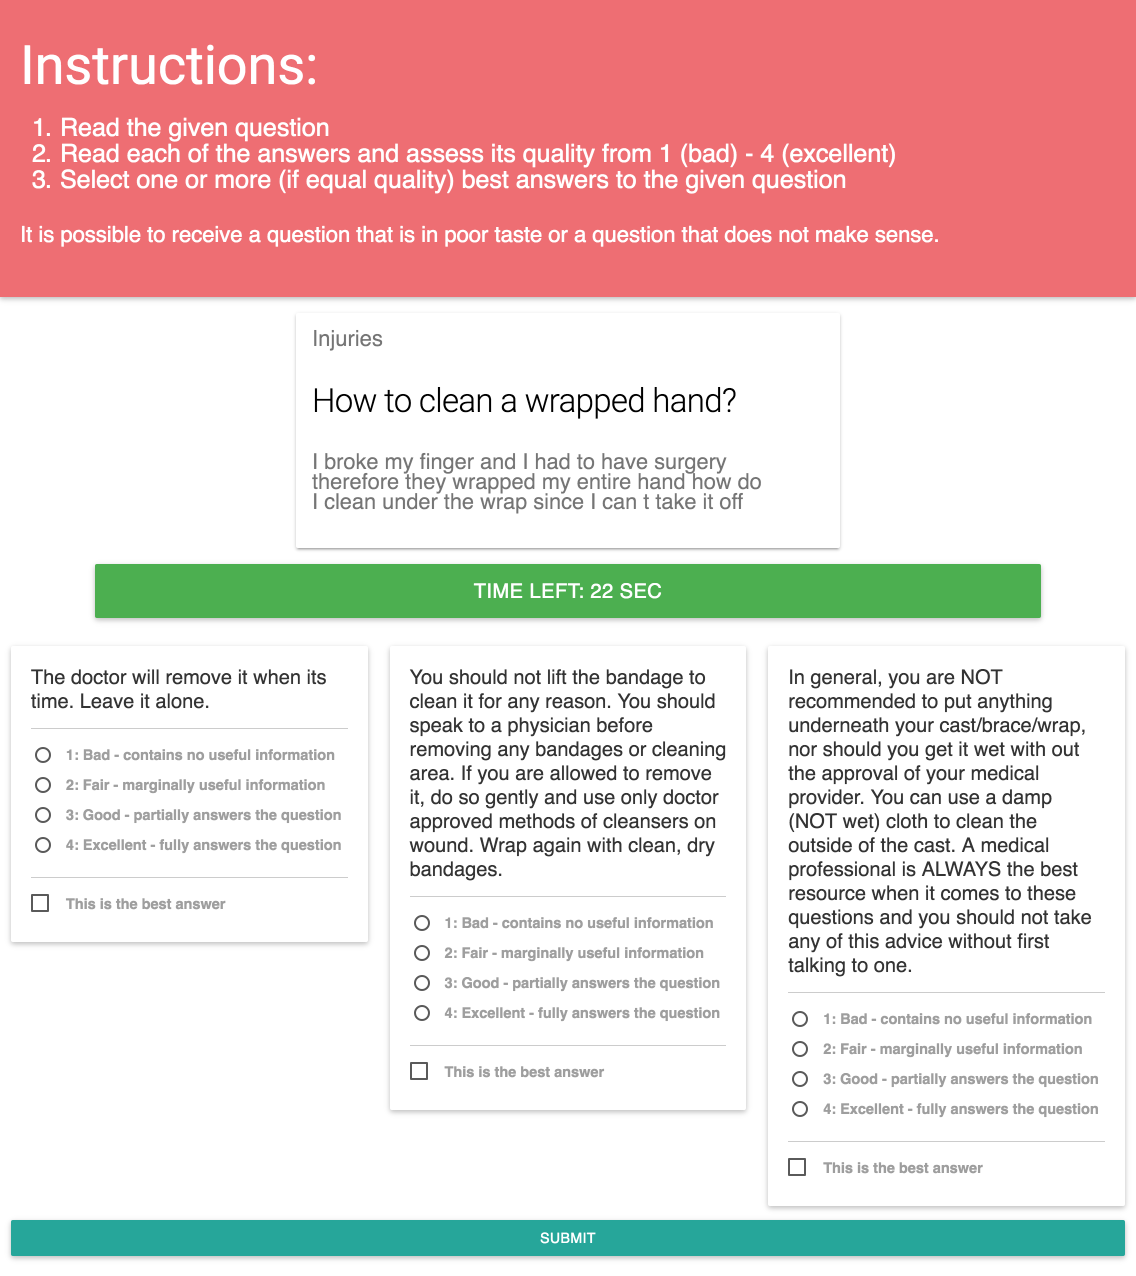
\includegraphics[width=\linewidth]{img/validation_screenshot}
\caption{Answer validation form}
\label{figure:crowdsourcing:interfaces:validation}
\end{subfigure}
\begin{subfigure}[b]{0.49\textwidth}
\centering
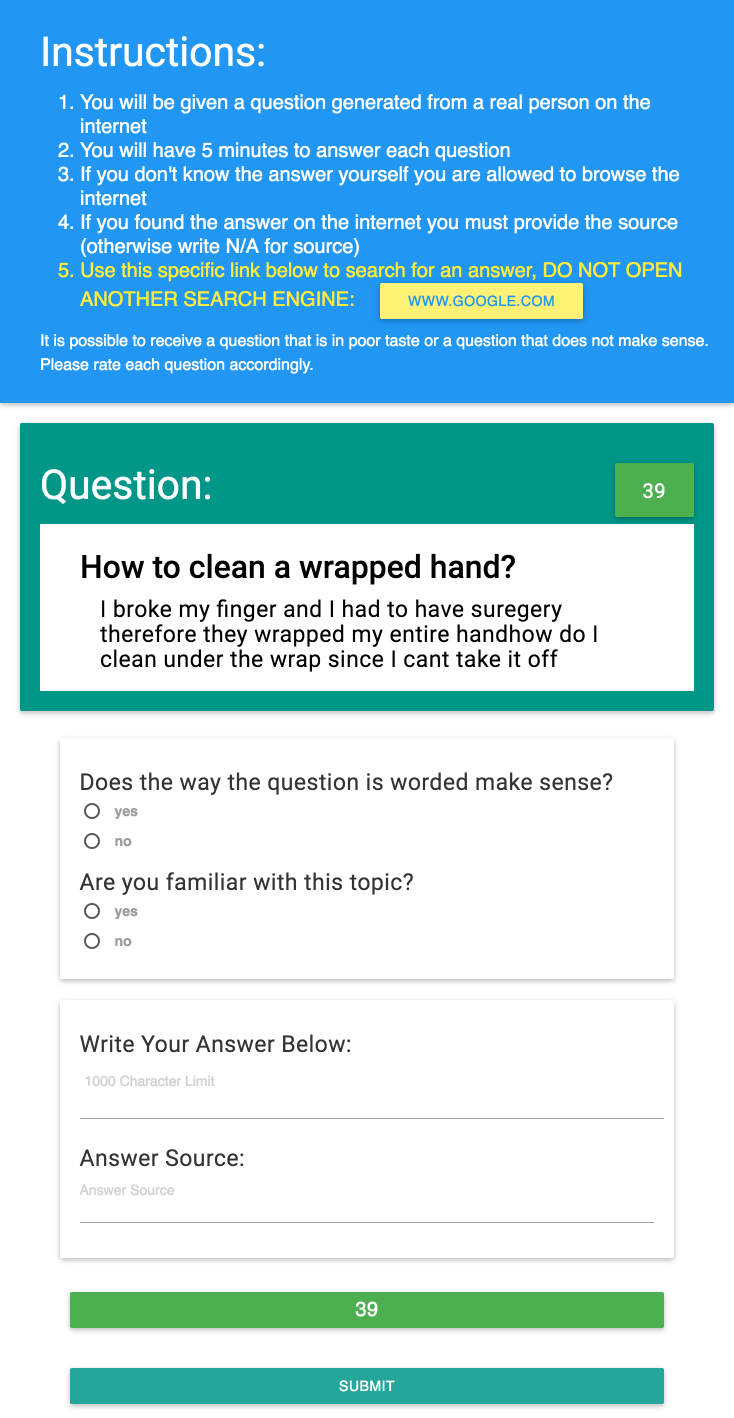
\includegraphics[width=0.9\linewidth]{img/answering_screenshot}
\caption{Answer crowdsourcing form}
\label{figure:crowdsourcing:interfaces:answer}
\end{subfigure}

\caption{Crowdsourcing user interfaces}
\label{figure:crowdsourcing:interfaces}
\end{figure*}

We chose to display 3 answers for a question, which were generated by three of the top-10 automatic systems from TREC LiveQA 2015 evaluation \cite{overviewliveqa15}.
To study the effect of time pressure on the quality of judgments we split participants into two groups. One group made their assessments with a 1 minute countdown timer shown to them, while the other could complete the task without worrying about a time limit.
Within each group, we assigned three different workers per question, and the workers were compensated at a rate of \$0.05 per question for this task.

\subsubsection{Answer validation experiment}
\label{section:crowdsourcing:approach:experiments:validation}

The interface for collecting answer ratings is illustrated in Figure \ref{figure:crowdsourcing:interfaces:validation}\footnote{The screenshots show the final state of the form, as we describe later in this sections fields were unhidden step-by-step for proper timing of reading, answering and validation}.
On top of the interface workers were shown the instructions on the task, and question and answers were hidden at this time.
They were instructed to read the question, read the answers, and rate each answer's quality on a scale from 1 (Bad) to 4 (Excellent), and finally choose a subset of candidates that best answer the question.
Upon clicking a button to indicate that they were done reading the instructions, the question, a 60 second countdown timer and 3 answers to the question appeared on the screen.
At the 15 second mark the timer color changed from green to red.
In the experiments without time pressure the timer was hidden, but we still tracked the time it took for the workers to complete the task.

At the end, we collected 6 ratings (3 with and 3 without time pressure) for each of three answers for a sample of 100 questions, which makes it a total of 1800 judgments.
Each answer also has an official NIST assessor rating on the same scale.
Figure \ref{figure:crowdsourcing:score_correlation} shows correlation between official NIST assessor relevance judgments and ratings provided by our workers.
The Pearson correlation between the scores is $\rho=0.52$.
The distribution of scores shows that official assessors were very strict and assigned many extreme scores of 1 or 4, whereas mechanical turk workers preferred intermediate 2s and 3s.
The results did not show any significant differences between experiments with and without time pressure.
Figure \ref{figure:crowdsourcing:validation_time} shows that even though the median time to rate all three answers is around 22-25 seconds in both experiments, the upper bound is significantly lower in the experiment with the time pressure.

\begin{figure}
	\centering
	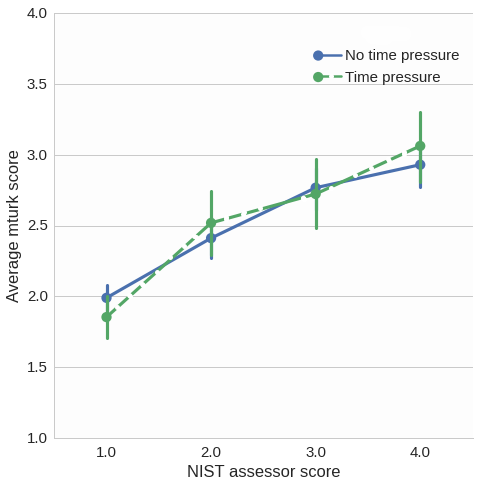
\includegraphics[width=0.35\textwidth]{img/score_correlation}
	\caption{Correlation between NIST assessor scores and crowdsourced ratings with and without time limit on the work time}
	\label{figure:crowdsourcing:score_correlation}
\end{figure}

\begin{figure}
	\centering
	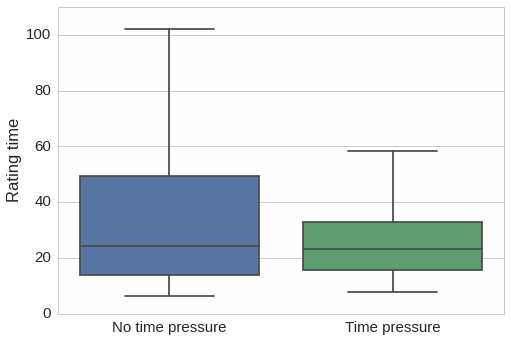
\includegraphics[width=0.4\textwidth]{img/validation_time}
	\caption{Box plot of answer rating time with and without time pressure}
	\label{figure:crowdsourcing:validation_time}
\end{figure}


Therefore, we conclude that in general we can trust crowdsourced ratings, and on average one minute is enough to judge the quality of three answers to CQA questions.

\subsubsection{Answer generation experiment}
\label{section:crowdsourcing:approach:experiments:generation}

In another experiment, designed to check whether crowd workers can provide an answer to a given question within a limited amount of time, we asked different workers to answer the questions from TREC LiveQA 2015.
We split the workers into two groups and displayed a one minute countdown timer for one of them.
We left a grace period and let the workers submit their answers after the timer had run out.
The workers received a \$0.10 compensation for each answer.
The form for answer crowdsourcing is shown in Figure \ref{figure:crowdsourcing:interfaces:answer}, and similar to the answer rating form, it starts with a set of instructions for the task.
We let the users browse the internet if they were not familiar with the topic or could not answer the question themselves.
To prevent them from finding the original question on Yahoo! Answers, we included a link to Google search engine with a date filter enabled\footnote{https://www.google.com/webhp?tbs=cdr:1,cd\_max:8/30/2015}.
Using this link, workers could search the web as it was on 8/30/2015, before TREC LiveQA 2015 questions were posted and therefore workers were in the same conditions as automatic systems on the day of challenge\footnote{The ranking of search results could be different on the day of the challenge and for our workers}.
Initially, the question was hidden for proper accounting of question-reading and answering times.
Upon clicking a button to indicate that they were done reading the instructions, a question appeared along with a button, which needed to be clicked to indicate that they were done reading the question.
After that, the answering form appears, it contained four fields:
\begin{enumerate}
\item Does the question make sense: ``yes'' or ``no'' to see if the question was comprehensible
\item Are you familiar with the topic: A yes or no question to evaluate whether the worker has had prior knowledge regarding the question topic
\item Answer: the field to be used for the user's answer to the given question
\item Source: the source used to find the answer: URL of a webpage or NA if the worker used his own expertise
\end{enumerate}

At the end, we collected 6 answers (3 with and without time pressure) for each of the 1087 LiveQA'15 questions.
Since we have answers from different sources, let's introduce the following notations:
\begin{itemize}
	\item \textit{Yahoo! Answers} - answers eventually posted by users on Yahoo! Answers for the original questions
	\item \textit{Crowd} - answers collected from Mechanical Turk workers without time pressure
	\item \textit{Crowd-time} - answers collected from Mechanical Turk workers with one minute time pressure
	\item \textit{LiveQA winner} - answers from the TREC LiveQA'15 winning system
	\item \textit{LiveQA top10} - answers from another top 10 TREC LiveQA'15 system.
\end{itemize}

Table \ref{table:crowdsourcing:answer_stats} summarizes some statistics on the answers.
The first thing to notice is that, unlike CQA websites, where some questions are left unanswered, by paying the crowd workers we were able to get at least one answer for all LiveQA questions (after filtering ``No answer'' and ``I do not know'' kind of responses).
The length of the answers, provided by Mechanical turk users is lower, and time pressure forces users to be even more concise.
The majority of workers ($\sim90 \%$) did not use the web search and provided answers based on their experience, opinions and common knowledge.

\begin{table*}[ht]
\centering
\begin{tabular}{| p{3cm} | c | c | c | c |}
\hline
Statistic & Y!A & mTurk & mTurk-time & LiveQA'15 winning system\\
\hline
\% answered & 78.7\% & 100.0\% & 100.0\% & 97.8\% \\
Length (chars) & 354.96 & 190.83 & 126.65 & 790.41 \\
Length (words) & 64.54 & 34.16 & 22.82 & 137.23 \\
\hline
\end{tabular}
\caption{Statistics of different types of answers for Yahoo! Answers questions}
\label{table:crowdsourcing:answer_stats}
\end{table*}

From Figure \ref{fig:answering_time_distribution} we can see that adding time pressure shifts the distribution of answering times\footnote{We had separate timers for reading the instructions, the question, and writing the answer, the inclusion of instruction-reading time is why the total time could be more than 1 minute}.
The tail of longer work times for no time limit experiment becomes thin with time restrictions and the distribution peaks around one minute.

\begin{figure}[t!]
	\centering
	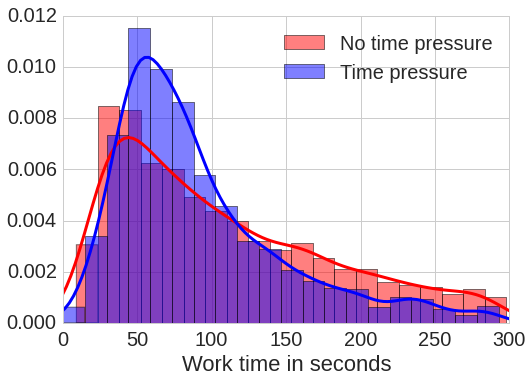
\includegraphics[width=0.4\textwidth]{img/answering_time_distribution}
	\caption{Distribution of answering times for experiments with and without time pressure}
	\label{fig:answering_time_distribution}
\end{figure}

\subsubsection{Answer quality comparison}
\label{section:crowdsourcing:approach:experiments:comparison}

Finally, to compare the quality of the collected answers with automatic system and CQA responses we pooled together the crowdsourced answers, the answers from the winning and other top-10 LiveQA'15 systems, and the original answers crawled from Yahoo! Answers.
We took a sample of 100 questions and repeated the answer rating experiment on this data.
Each answer was judged by 3 different workers (without time pressure), and their scores were averaged.
Figure \ref{figure:crowdsourcing:average_score} displays the plot with average score for answers from different sources.
Quite surprisingly the quality of collected answers turned out be comparable to those of CQA website users.
Average rating of answers produced by the winning TREC LiveQA system is also pretty close to human answers.
Finally, as expected, time pressure had its negative effect on the quality, however it is still significantly better than quality of an average top 10 QA system.

\begin{figure}[h]
	\centering
	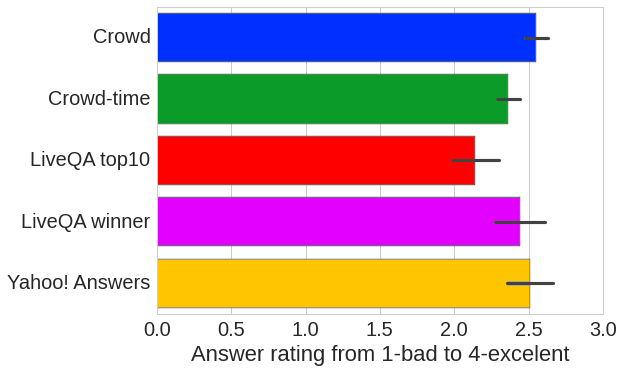
\includegraphics[width=0.4\textwidth]{img/average_score}
	\caption{Average scores of different types of answers to Yahoo! Answers questions}
	\label{figure:crowdsourcing:average_score}
\end{figure}

\begin{figure}[h]
	\centering
	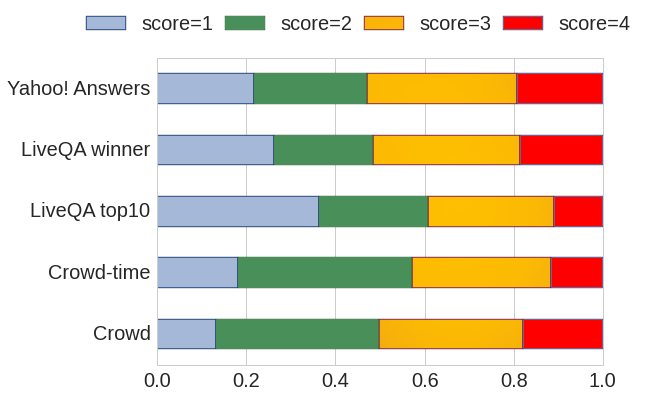
\includegraphics[width=0.4\textwidth]{img/scores_distribution}
	\caption{Distribution of scores for different types of answers to Yahoo! Answers questions}
	\label{figure:crowdsourcing:scores_distribution}
\end{figure}


Analysis of the score distribution (Figure \ref{figure:crowdsourcing:scores_distribution}) sheds some light on the nature of the problems with automatic and human answers. The automatic systems generate non-relevant answers ($score=1$) more often than human, either because the systems fail to retrieve relevant information, or to distinguish between useful and non-useful answer candidates. However, by having a larger information store, e.g., the Web, automated QA systems can often find a perfect answer ($score=4$), while crowd workers tend to give generally useful, but less perfect responses ($score=2,3$).

Our results suggest that the ``crowd'' can quickly give a reasonable answer to most CQA questions. However, some questions require a certain expertise, which a common crowd worker might not possess.
One idea to tackle this challenge is to design a QA information support system, which a worker can use to help them find additional information.
For example, in our experiment, we let workers use web search to find answers, if they were unfamiliar with the topic; more effective search interfaces may be helpful.

The findings of these experiments were used to implement our CRQA system, which stands for Crowd-powered Real-time Question Answering.
CRQA integrates a crowdsourcing module into an automated question answering system within an overall learning-to-rank framework for selecting answers to complex questions.
We report extensive experiments of stress-testing the CRQA system, by participating in the TREC LiveQA 2016 evaluation challenge, which provided us with a realistic evaluation setup.


\subsection{CRQA: Crowd-powered Real-time Automated Question Answering System}
\label{section:crowdsourcing:approach:crqa}

Our CRQA system represents a hybrid system, that includes an automated question answering and crowdsourcing modules.
The high level architecture is presented in Figure~\ref{figure:crowdsourcing:system}.

\begin{figure*}[h!t]
	\centering
	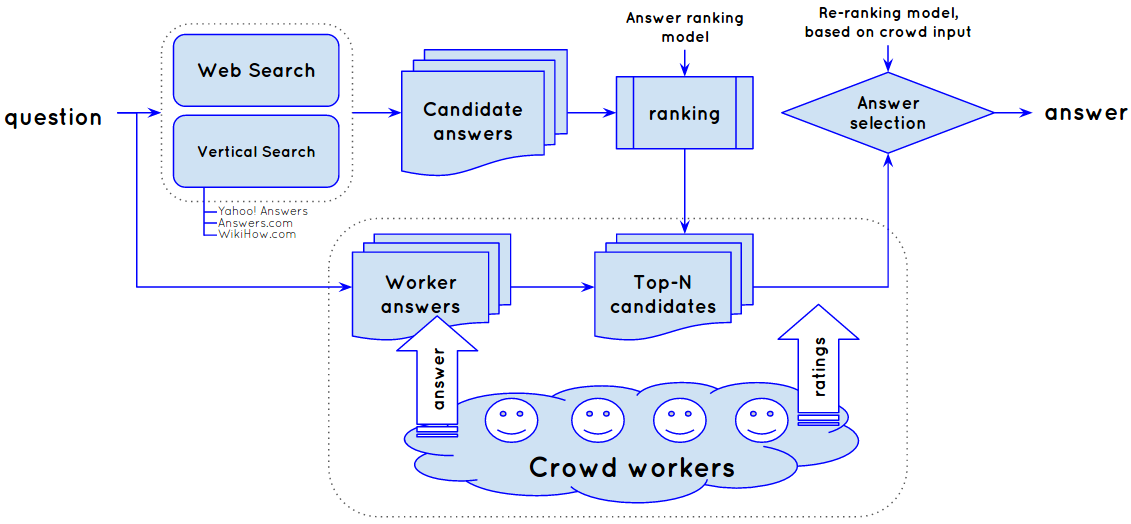
\includegraphics[width=\textwidth]{img/crqa_system}
	\caption{The architecture of our Crowd-powered Real-time Question Answering system, that uses crowdsourcing to augment a list of automatically extracted candidate answers and to rate their quality}
	\label{figure:crowdsourcing:system}
\end{figure*}

The automated part of the CRQA system follows an Information Retrieval (IR) approach to question answering, and generates a set of candidate answer passages from multiple data sources.
After candidates are generated, they are ranked by a trained model, and in the fully automated mode the top candidate could be returned as the answer.
The crowdsourcing module is designed to overcome two of the most common problems of the automated QA approaches: lack of good candidate answers and ranking errors.
More particularly, CRQA asks crowd workers to provide answers to the given questions if they can, and additionally rate the quality of candidate answers, generated by the automated system.
Worker contributions are then used by a trained re-ranking model, that selects the best candidate answers using all the information available.
The next two sections describe the architectures of the automated and crowdsourcing modules of our system.

\subsubsection{Automated question answering module}
\label{section:crowdsourcing:approach:crqa:auto}

When CRQA receives a question, it generates a set of search queries to retrieve a set of relevant documents and extract candidate answer passages.
Search queries are generated using the following strategies:
\begin{itemize}
\item Question title, which most often captures the gist of the question
\item Two longest question sentences (detected by the presence of the question word at the beginning or question mark at the end of a sentence) from the title and body of the question. In some cases the real user question is hidden inside the body, while the title just provides the overall topic of the question.
\item Concatenation of the question word, verbs and top-5 terms from the question title by Inverse Document Frequency\footnote{IDF of terms are estimated using Google N-gram corpus: https://catalog.ldc.upenn.edu/LDC2006T13}. This strategy targets over-specific questions, which often retrieve few if any search results.
\end{itemize}

To retrieve a set of potentially relevant documents and extract candidate answer passages, CRQA relies on multiple different generic and CQA document collections.
Previous research \cite{Shtok:2012:LPA:2187836.2187939} has shown that many of the user information needs are repeated, and reusing answers to previously posted similar questions is an effective strategy for answering new questions.
Therefore, CRQA uses multiple different CQA data sources, which potentially contain a diverse set of questions.
However, quite often it is hard to find a similar question in an archive, and many of the information needs are unique.
Therefore, we include a web search component, that can retrieve regular web documents, from which our system can extract candidate answers.
More specifically, CRQA queries the web using Bing Web Search API\footnote{https://datamarket.azure.com/dataset/bing/searchweb}, Yahoo! Answers, Answers.com and WikiHow.com using their respective search interfaces.
For each query we retrieve top-10 relevant documents and question-answer pairs from CQA archives.
As candidate answers CRQA extracts answers to the questions retrieved from CQA results and paragraphs of text from the main content of regular web documents, as detected by a method based on \cite{Kohlschutter_2010}.
Quite often, it is hard to estimate the quality of a candidate answers from its text only.
The task becomes much easier if a system has access to additional data, \eg for the candidates generated from the CQA archives, it is useful to know the text of the original question the candidate answers.
For candidates, generated from regular web pages, it is useful to know the topic of the page (\eg from its title), additionally the context of the candidate, such as text that immediately precedes it in the document was shown to provide a useful information for QA.
Therefore, besides the text of a candidate answer, we keep some potentially useful metadata, \eg for QnA candidates we include text and category of the retrieved question, and web page title and text block preceding the answer passage in the document for web-search based candidates.
For convenience, we will call the title of a retrieved question or web page \textit{``the answer topic''}, and the body of the retrieved question or the preceding text block the \textit{``the answer context''}.

Next, for each candidate answer we compute a set of features, described in Table \ref{table:crowdsourcing:crqa:features}.

\begin{table}[ht]
\centering
\begin{tabular}{| p{12cm} |}
\hline
\textbf{Answer statistics} \\
\hline
--- Length in chars, words and sentences \\
--- Average number of words per sentence \\
--- Fraction of non-alphanumeric characters  \\
--- Number of question marks \\
--- Number of verbs  \\
\hline
\textbf{Answer source} \\
\hline
--- Binary feature for each of the search verticals: Web, Yahoo! Answers, Answers.com, WikiHow.com \\
\hline
\textbf{N-gram matches}\\
\hline
--- Cosine similarities using uni-, bi- and tri-gram representations of the question title and/or body, and answer text, topic or context\\
--- The lengths of longest spans of matched terms between question title and/or body, and answer text, topic or context\\
\hline
\textbf{Information Retrieval score}\\
\hline
--- BM25 scores between question title and/or body, and answer text, topic or context\\ 
\hline
\end{tabular}
\caption{The list of candidate answer ranking features used by the automated module of our CRQA system}
\label{table:crowdsourcing:crqa:features}
\end{table}

The final stage of the module is answer ranking, where a trained LambdaMART \cite{burges2010ranknet} model sorts the candidates by their predicted quality.
This model was trained using the RankLib library\footnote{https://sourceforge.net/p/lemur/wiki/RankLib/} on the data from last year TREC LiveQA task\footnote{https://sites.google.com/site/trecliveqa2016/liveqa-qrels-2015}, which includes 1087 questions with answers provided by the participants, each of which was rated on a scale from 1(bad) to 4(excellent) by professional NIST assessors.
In a fully automated setup the top candidate could be returned as the final answer to the question, but in this work we explore if we can further improve the performance of the system using crowdsourcing.

\subsubsection{Crowdsourcing module}
\label{section:crowdsourcing:approach:crqa:crowdmodule}

As we mentioned before, two of the main problems with the fully automated system responses are lack of good candidates and problems with ranking, therefore, we decided to explore if crowdsourcing can be helpful to overcome these challenges in near real-time scenario.
Instead of returning the final answer, the system sends the question and top-7 ranked candidates to the crowd workers and waits for the responses.
We chose to give 7 answers based on the average number of rated answers in our preliminary studies.
Since systems had only 60 seconds to answer each question, we start a timer when a question arrives, and the system waits to receive all worker contributions until the timer reaches 50 seconds to leave the system some time to generate the final answer and minimize the chances of going above the time limit.
CRQA asks workers to write their own answers to questions if possible, which should provide additional candidates in case there are no good automatically generated ones.
Additionally, systems expects workers to rate the quality of top-7 ranked candidates, which should help to fix the ranking problems and select a better final answer.
Figure~\ref{figure:crowdsourcing:crowd_ui} presents the user interface of our crowdsourcing module.

\begin{figure*}[h!t]
	\centering
	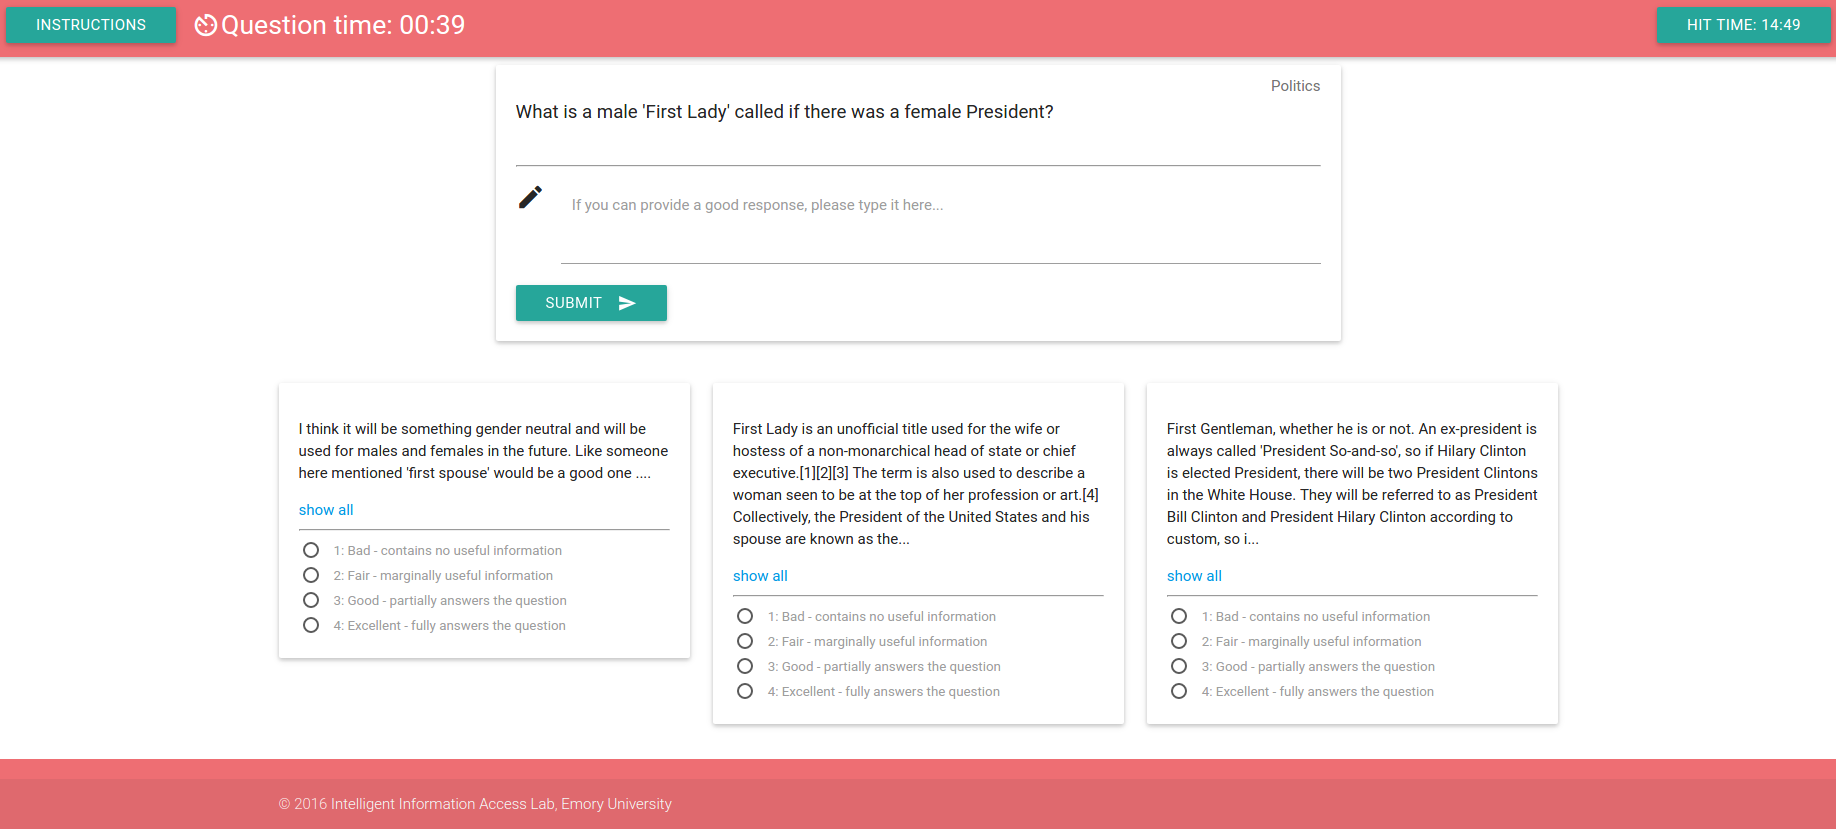
\includegraphics[width=\textwidth]{img/crqa_crowd_ui}
	\caption{User Interface for workers in our Crowd-Powered Question Answering system}
	\label{figure:crowdsourcing:crowd_ui}
\end{figure*}

The overall algorithm for obtaining crowd input for real-time question answering is the following:
\begin{enumerate}
\item When a system receives a question, it is posted to the workers, who will have 50 seconds to provide their input
\item Workers are asked to write an answer if they can provide one (it is optional)
\item Otherwise they are waiting for the answer candidates to arrive
\item When a system is done with generating and ranking candidates it posts top-7 scoring answers to the workers for the rating (which usually leaves $\sim$ 35 seconds for rating)
\item Workers receive a list of answers\footnote{Answers submitted by workers are also sent for ratings to all workers except the author} and rate them until the timer runs off. Each answer is rated on a scale from 1 to 4, using the official TREC LiveQA rating scale:
	\begin{itemize}
    \item 1 --- Bad: contains no useful information
    \item 2 --- Fair: marginally useful information
    \item 3 --- Good: partially answers the question
    \item 4 --- Excellent: fully answers the question
    \end{itemize}
\item The interface displays 3 answers at a time, when an answer gets rated, it disappears and its place is taken by another answer from the pool. The interface displays only the first 300 characters of the answer, which was experimentally shown to be enough on average to make a good judgment.
Full answer can be revealed upon clicking the ``show all'' link.
\item When the timer runs off, the question and all the answers disappear, and workers wait for the next question
\end{enumerate}

% Not sure we need a title, as this subsection already describes the crowdsourcing module.
% \noindent\textbf{QARC system implementation: Crowd module}:
To hire the workers we used Amazon Mechanical Turk platform\footnote{http://mturk.com}.
Since the challenge was to run the system ``live'' over the period of 24 hours, we adapted the ``retainer'' model to our question-answering task, inspired by the success of this model reported in previous work \cite{bernstein2011crowds,bigham2010vizwiz}.
Specifically, to obtain an even distribution of workers over the 24-hour period of the TREC LiveQA shared task, we posted 10 tasks every 15 minutes, and they expired after the next set of tasks became available.
Since not all assignments were accepted by some worker right away, the number of workers for each question varied and could be greater than 10.
When a worker first gets to our crowdsourcing interface, she is shown task instructions (Table \ref{table:crowdsourcing:crqa:crowd_instructions}) and asked to wait for the questions to arrive.
The workers were paid \$1.00 for the whole 15 minutes task, no matter how many questions they got\footnote{In TREC LiveQA task questions are sent to the systems one by one, therefore there is no concurrency, however the delays between the questions are possible}.

\begin{table}[ht]
\centering
\begin{tabular}{| p{15cm} |}
\hline
\textbf{Instructions} \\
\hline
1. This HIT will last exactly 15 minutes\\
2. Your HIT will only be submitted after these 15 minutes\\
3. In this period of time you will receive some questions, that came from real users on the Internet\\
4. Each question has a time limit after which it will disappear and you will need to want for the next one\\
5. If you know the answer to the question, please type it in the corresponding box\\
6. At some point several candidate answers will appear at the bottom of the page\\
7. Please rate them on a scale from 1 (bad) to 4 (excellent)\\
8. Do not close the browser or reload the page as this will reset your assignment.\\
\hline
\end{tabular}
\caption{Crowdsourcing task instructions, displayed to the user when she first gets to the task}
\label{table:crowdsourcing:crqa:crowd_instructions}
\end{table}

\textbf{Answer re-ranking and selection}.
The last stage in CRQA is answer re-ranking, which aggregates all the information received from the crowdsourcing and produces the final answer to the question.
The input of the re-ranking module is a set of candidate answers with quality ratings provided by the crowd workers.
Candidates can include the answers posted by the workers, which might also be rated, if workers had enough time to do that.
To re-rank the answers we trained a gradient boosting regression trees (GBRT) model \cite{friedman2002stochastic}.
To build this model we used a training set of questions with answers generated by our system.
The quality of each answer was manually assessed using the official LiveQA scale from 1 (bad) to 4 (excellent).
The features, used for answer re-ranking are listed in Table~\ref{table:crowdsourcing:crqa:reranking_features}.

\begin{table}[ht]
\centering
\begin{tabular}{| p{15cm} |}
\hline
\textbf{Answer-based} \\
\hline
--- The length of the answer \\
--- Source of the answer (Crowd, Web, Yahoo! Answers, Answers.com or WikiHow.com)\\
--- Original rank of the candidate answer or -1 for answers provided by the crowd workers\\
\hline
\textbf{Worker ratings} \\
\hline
--- Number of ratings provided\\
--- Minimum, maximum, median and average ratings\\
\hline
\end{tabular}
\caption{The list of features used for answer re-ranking based on crowdsourcing input}
\label{table:crowdsourcing:crqa:reranking_features}
\end{table}

CRQA sorts the candidates by the quality score predicted by the model, as returns the top candidate as the final answer.


\subsubsection{Experiments}
\label{section:crowdsourcing:approach:crqa:experiments}


We now describe the experimental setup used to evaluate the performance of CRQA and other methods for near real-time question answering.

The experimental evaluation of our CRQA system was done on the official run of TREC LiveQA shared task, which happened on May 31, 2016.
All participating systems were running for 24 hours and received questions sampled from the live (real-time) stream of questions, posted by real users to Yahoo! Answers platform.
In total, each system received 1,088 questions, and system responses were recorded by the organizers.

\begin{table}[ht]
\centering
\begin{tabular}{| p{14cm} | c | }
\hline
Name & Value \\
\hline
Number of questions received & 1088 \\
Number of completed assignments (15 mins each) & 889 \\
Average number of questions per assignment & 11.44 \\
Total cost per question & \$0.81 \\
Average number of answers provided by workers & 1.25 \\
Average number of ratings per answer & 6.25 \\
\hline
\end{tabular}
\caption{Aggregate statistics of crowdsourcing tasks}
\label{table:crowdsourcing:crqa:task_stats}
\end{table}

Overall statistics are provided in Table~\ref{table:crowdsourcing:crqa:task_stats}.
As we can see, on average workers were able to provide at least one answer for each question, and each of the provided answers got 6 ratings.
Since the interface could show only 3 answers at a time, answers had different chances of being rated.
To investigate the effect of the order of the candidates posted for ratings on the quality of the final answer, in CRQA for each worker and each question we randomly selected one of the strategies: ordering answer candidates by their model rank or random shuffling of the candidates.
The system variant with shuffled candidates for rating was expected to obtain more diverse and comprehensive set of ratings, as we will investigate in the Analysis section.

The official results of the shared task will be available in November 2016 during the TREC conference\footnote{http://trec.nist.gov/}.
Meanwhile, we used traditional (batch-mode) crowdsourcing to obtain the quality labels for all answer candidates that were given to the workers during the task, as well as the answers provided by the workers.
In addition, on June 2, two days after the TREC LiveQA challenge has completed, we crawled the current answers provided by the community for the questions, used for the task.
All the answers for each question were randomly shuffled and rated on a scale from 1 (bad) to 4 (excellent) by workers hired on Amazon Mechanical Turk.
As we have shown in the previous section, crowdsourced labels correlates well with the official ratings, provided by the professional NIST assessors.
Each answer was labeled by 3 different workers, and we averaged the scores to get the final quality labels for the candidates.

We compared CRQA system against several baselines:
\begin{itemize}
\item \textit{Automated QA}: automated QA system described in Section~\ref{section:crowdsourcing:approach:crqa:auto}.
\item \textit{CRQA}: Automated QA system with Crowdsourcing, described in Section~\ref{section:crowdsourcing:approach:crqa:crowdmodule}
\item \textit{Re-ranking by score}: a simplified version of CRQA re-ranking model, which select the answer with the highest average ratings, provided by the crowd workers.
\item \textit{Yahoo Answers}: traditional, non-real-time community question answering site (Yahoo Answers), from which the challenge question originated. The answers were collected two days after the challenge, thus allowing the Yahoo Answers community extra two days to collect the answers through traditional (community-based) crowdsourcing.
\end{itemize}

To evaluate the methods we used the metrics proposed by the organizers of the LiveQA task:
\begin{itemize}
\item \textbf{avg-score}: average score over all questions
\item \textbf{avg-prec}: average score over all answered questions
\item \textbf{s@i+}: the fraction of answers with score i or greater (i=2..4)
\item \textbf{p@i+}: the number of answers with score i or greater (i=2..4) divided by the number of answered questions\footnote{Since for each answer we averaged 3 ratings by different workers, the number of answers with the average score of 4 is low}
\end{itemize}

\begin{table*}[ht]
\centering
\begin{tabular}{| p{4.2cm} | c | c | c | c | c | c | c | c |}
\hline
Method & avg-score & avg-prec & s@2+ & s@3+ & s@4+ & p@2+ & p@3+ & p@4+ \\
\hline
Automated QA & 2.321 & 2.357 & 0.697 & 0.297 & 0.026 & 0.708 & 0.302 & 0.026 \\
Re-ranking by score & 2.416 & 2.421 & 0.745 & 0.319 & 0.031 & 0.747 & 0.320 & 0.031 \\
Yahoo! Answers & 2.229 & 2.503 & 0.656 & 0.375 & \textbf{0.045} & 0.737 & \textbf{0.421} & \textbf{0.050} \\
CRQA & \textbf{2.550} & \textbf{2.556} & \textbf{0.799} & \textbf{0.402} & 0.034 & \textbf{0.800} & 0.402 & 0.034 \\
\hspace{5mm}worker ratings only & 2.432 & 2.470 & 0.750 & 0.348 & 0.030 & 0.762 & 0.354 & 0.031 \\
\hspace{5mm}worker answers only & 2.459 & 2.463 & 0.759 & 0.354 & 0.029 & 0.760 & 0.355 & 0.029 \\
\hline
\end{tabular}
\caption{Evaluation of the baselines and system answers quality based on the ratings of answers obtained via crowdsourcing. The scores are averaged over 100 different 50:50 splits of 1088 questions into the training and test set. The differences between average score and precision of CRQA and the original ranking are significant at p-value $<$ 0.01}
\label{table:crowdsourcing:crqa:performance}
\end{table*}

Table~\ref{table:crowdsourcing:crqa:performance} summarizes the performance of the baselines and our system.
As we can see, the average score and precision of answers generated by CRQA system is higher than the baseline ranking and even community answers on the Yahoo! Answers platform.
However, Yahoo! Answers community answers have higher percentage of \textit{``4 (excellent)''} scores.
Figure \ref{figure:crowdsourcing:crqa:score_histogram} shows the distribution of scores for the original system ranking, our crowdsourcing system and Yahoo! Answers.
Two peaks on the distribution of scores from Yahoo! Answers community suggest, that there are essentially two kinds of responses: non-useful (\eg spam) or excellent that fully answers the question.
In addition, around 20\% of the questions did not get any answer from the community.
Automatically generated answers, on the contrary, are rarely empty, but on average provide only marginally relevant information, which often does not answer the questions, and therefore rated \textit{``2 (fair)''}.
The introduction of the crowdsourcing module allowed CRQA to cover a couple of percent of the questions, for which the automated system was not able to generate any candidates, as well as select better candidates when it was possible using crowd ratings.

\begin{figure}[h]
	\centering
	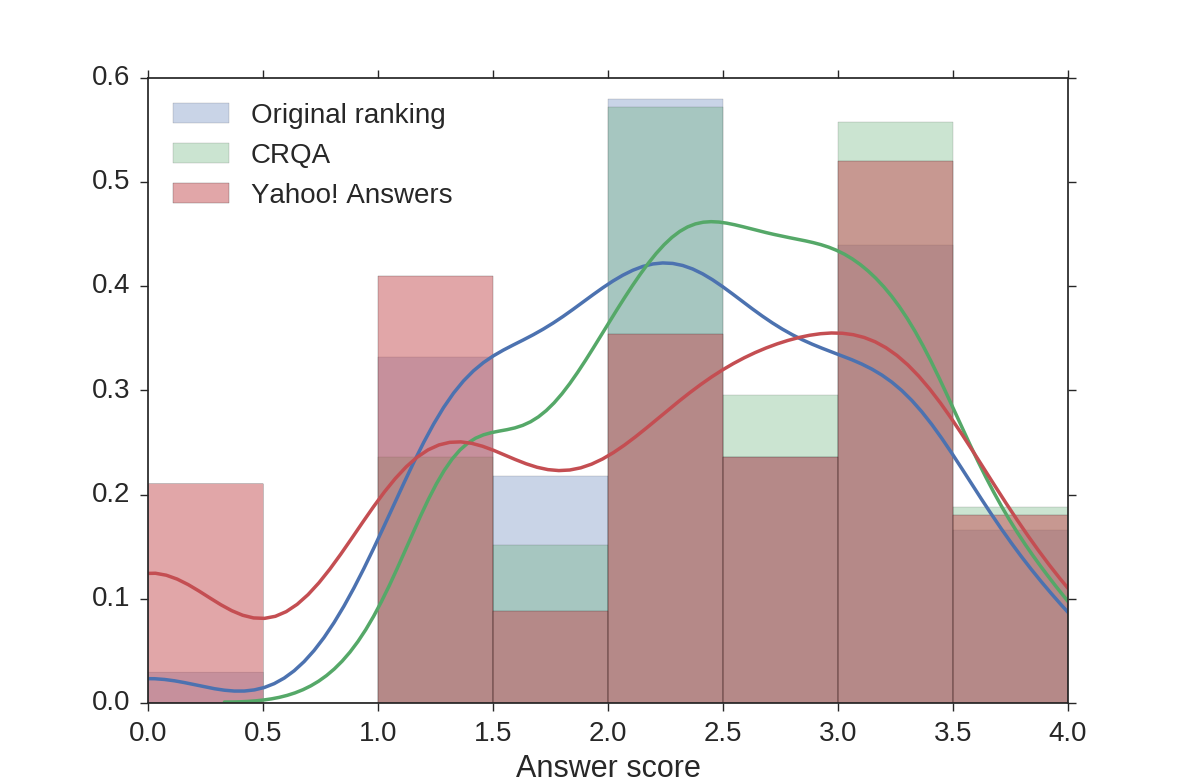
\includegraphics[width=0.5\textwidth]{img/crqa_score_hist}
	\caption{Histogram and kernel density estimation of answer scores for original candidate ranking, CPQA model re-ranking and Yahoo! Answers answers}
	\label{figure:crowdsourcing:crqa:score_histogram}
\end{figure}

Therefore, we can conclude, that crowdsourcing can effectively help automated QA system to improve the performance of question answering, by providing worker generated answers and rating existing candidates.

\subsubsection{Analysis}
\label{section:crowdsourcing:approach:crqa:analysis}

In this section we will analyze some of the results of our experiments and discuss their implications.

\textbf{Worker answers vs ratings}.
First, let's look at the contribution of additional answers and answer ratings provided by the workers.
These two types of contributions are complimentary to each other and attempts to solve different problems.
Table \ref{table:crowdsourcing:crqa:performance} shows the performance of our question answering system using each of these types of feedback independently.
The results demonstrate that both answers and ratings have positive effect on the performance.
Even with limited time, workers were able to reliably rate candidate answers, which helped the system to select a better final answer and improve the model precision.
However, this method does not help the system in cases, when it was not able to generate a good candidate in the first place, therefore using ratings only has lower average answer score than using worker generated answers.
By asking the crowd to provide a response if they can answer the question, CRQA covers this gap, which is important as in a real scenario even a fair answer would probably be better for the user than no answer at all.
Of course, given limited time and the fact that a random worker might not possess an expertise required to answer the question, such answers do not always perfectly answer the question.
Table \ref{table:crowdsourcing:crqa:answer_examples} gives some examples of worker generated answers with low and high quality scores.

To summarize, ratings of answer candidates and worker generated answers both have similar positive effect on the performance of our question answering system.
What is more important, the contributions are independent and therefore it is beneficial to use both of them in the final system.

\begin{table*}[ht]
\centering
\begin{tabular}{| p{10.5cm} | p{5cm} | c |}
\hline
Question & Answer & Score \\
\hline
 Is Gotu Kola a good herb for mental health? How long does it take to work?? & yes & 1.66\\
 \hline
Can I write any number on line number 5 of a W2?  would like to set up my W2 were I get the most out of my paycheck and not have to pay taxes at the end of the year... & W2 & 1.33\\
 \hline
I need help with my mum? Something traumatic happened to me about 4 years ago i randomly asked my mother why when I lived with you in your home country a man that was our neighbour used to call me his daughter and the younger kids that lived there called me there cousins and one boy called me his sister? & yes & 1.0\\
\hline
\hline
 Is it bad not wanting to visit your family? & It is nt bad. Just be honest with them. They may be upset but they should understand & 3.0 \\
 \hline
Any health concerns with whey protein? So I workout 3-5 days a week and i drink a whey protein isolate after each workout. Since I workout almost everyday, is it ok for me to just drink a shake everyday?.. & As long as you use it as directed, there should not be any major problems.  You may want to consult your doctor just in case, but I would not be too concerned. & 3.0\\
\hline
Foot pain unable to walk? Hi so today woke with some pain, I am able to put weight on my heel with no problem or pain.  But  the area between my heel and toes hurts really bad when I try to go with the motion of taking a step. Its not swollen and I do not remember hurting it at all & Possible gout in your foot, also possible you may have strained it during the previous day. & 3.0\\
\hline
What is a good remedy/medicine for stomach aches? Specifically ones caused by stress or anxiety? & Chamomile tea should help & 3.66\\
\hline
\end{tabular}
\caption{Examples of answers provided by the crowd workers and their average quality scores}
\label{table:crowdsourcing:crqa:answer_examples}
\end{table*}

\textbf{Selection of answer candidate for rating}.
Predicting the quality of answers and ranking them to select the best is one of the main challenges in automated question answering \cite{surdeanu2011learning}.
External feedback, such as noisy answer ratings, obtained from the crowd workers, provide valuable information, which, as our results demonstrate, can help a QA system to better re-rank the answers.
However, the capacity of crowdsourcing for answer ratings are obviously limited, as systems often are dealing with hundreds and thousands of answer candidates for a given question.
In this work, we made a choice to rate only top-7 answers according the automated system ranking.
This decision was made based on the average number of ratings workers could provide in the allotted time\footnote{The answers were posted for rating automatically after an automated system was done with candidate generation and ranking. On average users had $\sim$ 35 seconds to provide the ratings.}.
However, the order in which the answers are shown can also have a strong effect on the system performance, because the answers are typically rated one by one in the order they are displayed on the screen.
Our system included two strategies for answer ordering: random or according to their ranking score.
The former strategy provides a uniform coverage for all the answers selected for rating, while the later puts more emphasis on the currently top scoring candidates.
We randomly selected one of the strategies for each user and question.
To analyze the performance of each of the strategies we compute the average score of answers, generated using the corresponding ratings.
The average score for answers generating when candidates are shuffled is 2.508, and it is 2.539 when the candidates are sorted according to their model ranking score.
This suggests, that it is beneficial to allocate more of the workers attention on the top scoring candidate answers.

\textbf{Cost analysis}.
The results of our experiments clearly demonstrated that crowdsourcing can improve the performance of near real-time question answering system.
The next reasonable question is what is the price of this improvement.
In our study we paid workers \$1.00 per single 15 minutes task, and each 15 minutes we had 10 assignments, which translates to \$15.00 per 15 minutes.
Overall, our experiment cost \$0.88 per question, and in this section we will discuss some ideas to reduce this cost.

First, we will study the effect of the number of workers on the performance of our CRQA system.
For this experiment we randomly sampled certain percentage of workers and removed all contributions (answers and ratings) of others.
Figure \ref{figure:crqa:nworkers_vs_quality} plots the dependency of the performance of our QA system on the number of workers.

\begin{figure*}[h!t]
  \begin{subfigure}[t]{0.5\textwidth}
	\centering
	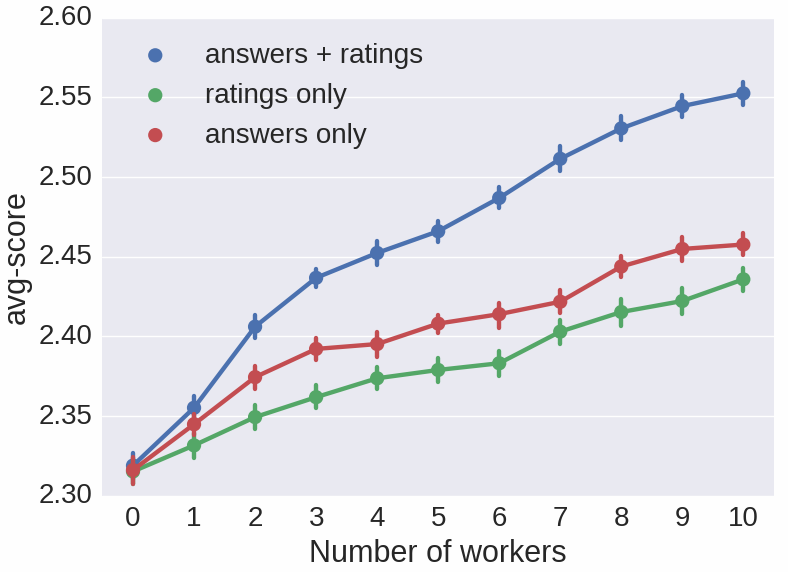
\includegraphics[width=\textwidth]{img/crqa_nworkers_vs_accuracy}
	\caption{avg-score: Average score per question}
	\label{figure:crqa:nworkers_vs_accuracy}
  \end{subfigure}
  \begin{subfigure}[t]{0.5\textwidth}
	\centering
	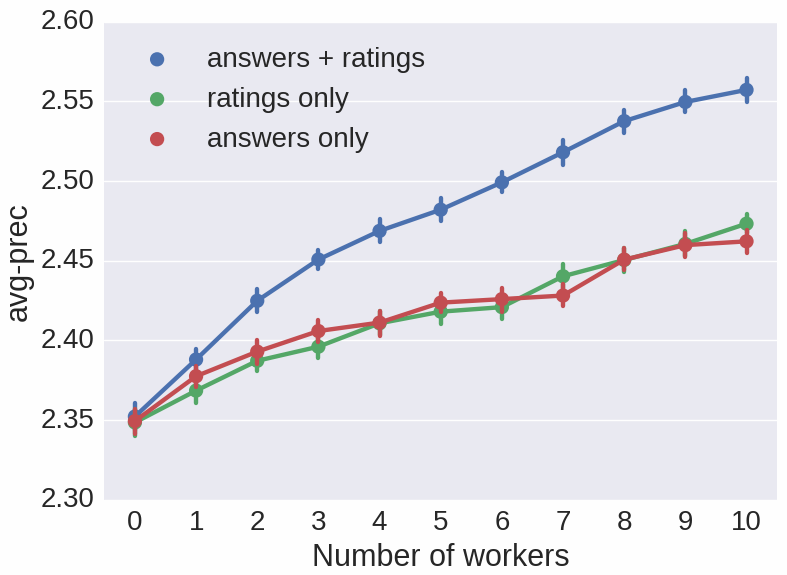
\includegraphics[width=\textwidth]{img/crqa_nworkers_vs_precision}
	\caption{avg-prec: Average score per answer (ignoring non-answered questions)}
	\label{figure:crqa:nworkers_vs_precision}
  \end{subfigure}
	\caption{Plot showing how the quality of the final answer depends on the number of workers per question}
	\label{figure:crqa:nworkers_vs_quality}
\end{figure*}

Obviously more workers mean more reliable answer ratings and more answer candidates, which improves the performance of the question answering system.
However, we can observe diminishing returns, as the cost per extra gain in performance metrics decreases as the number of workers grow.
Half of the overall performance improvement could be achieved with only 3 workers per question, which would save 70\% of the costs.

An alternative cost-reduction strategy is selective triggering of crowdsourcing, which would only ask for workers feedback for some of the questions.
Such a strategy would be necessary to scale a crowd-powered question answering system to a higher volume of questions.
There are multiple different approaches for such selective crowdsourcing: \eg a system can only ask for crowd contributions if it did not generate enough candidate answers or the predicted quality of the top scoring candidates is low \cite{carmel2010estimating,he2006query}.
We leave this questions for the future work, as here we focused on the scenario, proposed by the organizers of the TREC LiveQA shared tasks, where questions arrive one by one and it is possible to utilize crowd input for every questions.

To summarize, in the explored real-time QA scenario it is possible to reduce the costs of crowdsourcing by reducing the number of workers, although with some performance losses.
Our analysis suggests that paying 30\% of the original cost would give 50\% of the performance improvement.

\subsection{Summary}

In this section we presented CRQA, the first, as far as we know, real-time question answering system that integrated crowd work within an automated question answering system.
Specifically, we explore different methods of obtaining input from the crowd, and use a machine-learned answer re-ranking model that incorporates the crowd input as features to select the final system answer to return to the user. 

We report a large-scale experiment in which over a thousand real user questions were submitted to the CRQA system in real-time, as part of the LiveQA challenge.
CRQA was able to successfully answer these questions in under 1 minute, with over 80\% of the answers subsequently rated to be fair or better.
Importantly, CRQA significantly improved question quality and coverage compared to the starting automated-only system, and, surprisingly, was able to return better answers on average compared to the traditional CQA system with millions of users (Yahoo! Answers) with answers collected more than \textit{two days} after the original posting time.

The described CRQA implementation is a promising step towards efficient and close integration of crowd work and automated analysis for real-time question answering.
It raises many promising issues and opens directions for future work, such as selective crowdsourcing for only the questions deemed ``difficult'' for the automated system; more efficient online learning for obtaining ratings from the crowd and integrating them into the ranking model; and investigating additional features and sources of evidence for improving the joint ranking of the system and crowd input.
This section describes a flexible and powerful framework for combining the powers of crowdsourcing with automated question answering techniques, for building the next generation of real-time question answering systems.

\section{Proposed Directions for Future Research}
\label{section:crowdsourcing:proposal}

The results described above demonstrate how effective can crowdsourcing be for real-time question answering.
However, it can also be quite expensive, which is one of the most critical problems for scalability of hybrid system.
Such a system needs to have a good strategy to deal with increasing volume and velocity of the input data, \ie user questions.
CRQA system, developed to participate in TREC LiveQA cost us \$0.81 per question, which is quite expensive, and according to our analysis in Section~\ref{section:crowdsourcing:approach:crqa:analysis} it is possible to get half of the performance gain for 30\% of the costs by hiring less workers.
However, in general such a strategy is not agile enough, as some questions might be very easy and system do not actually need any worker input, while some others are very hard and would benefit from more human feedback.
In addition, in different situations our hybrid system might need different types of feedback, \eg for some questions some help with answer ranking is more important than additional candidates, and sometimes the opposite.

The research proposed below targets the problem of designing an optimal crowdsourcing plan, \ie allocation of crowdsourcing resources across different tasks.
The first step towards this goal is to develop a model for selective crowdsourcing, \ie identification of cases when an automated system would benefit from crowdsourcing the most and when it might be redundant.
Next, if a system decides to request feedback from crowdsourcing, we need to decide how much resources to allocate (number of workers and time) and where to target it (what kind of feedback to request from how many users).

% \todo{We also had an idea to utilize feedback more efficiently. The system might rerank all candidates based on feedback, or it can even request more candidates using worker feedback}
% \todo{User expertise and question routing, a lot of previous research. Except based on feedback a user provided, estimate her trustworthiness, expertese and whether she better rates or answers questions}

\subsection{Method}
\label{section:crowdsourcing:method}

First, we need to formulate the conditions and objectives of the problem we are trying to solve, \ie resource and quality conditions, etc.
An important problem to focus on in the future research is optimizing the quality of hybrid question answering under the fixed crowdsourcing budget.

A possible approach on the problem is to stick with the real-time scenario, proposed in TREC LiveQA challenge, and set the maximum response time to 1 minute after the question is posted.
In such scenario, for the selective crowdsourcing problem one can train a machine learning model to predict the expected performance of the answer, given all the current candidates.
This problem is very similar to search query performance prediction~\cite{carmel2010estimating,he2006query,zhou2007query}, and therefore we can adapt the ideas developed in this line of research.
More specifically, a machine learning model (\eg random forest or gradient boosted regression trees) can be trained to predict the expected relevance score of the answer a system is about to return, given the following set of features:
\begin{itemize}
\item single answer features: answer length, information retrieval score given the question text and other features used for answer ranking
\item results list features: syntactic and semantic similarity of the top answer to other retrieved candidates
\item corpus dependent features: query clarity score~\cite{cronen2002predicting}, which measures the coherence of the retrieved results (answer candidates) with respect to the whole corpus
\end{itemize}

In the simplest case, the score, returned by this model, can be thresholded to determine if the answers is expected to be good and no crowd feedback is needed, or if the system would benefit from worker contributions.
Alternatively, it is possible to experiment with adaptive thresholding, which can be implemented by putting all the questions into a single priority queue, based on their expected quality from lowest to highest.
The workers will be assigned to the tasks from the top of the queue, \ie starting from the lowest expected performance.
Decision on how many workers assign to which tasks depends on many factors, such as total number of workers available, number and expected performance of other questions expecting crowdsourcing feedback in the queue.
Therefore, to design a resource allocation strategy I will train another machine learning model, that will predict how much workers to assign to each question, given the total number of workers and information about the other questions waiting in the queue, \ie expected performances of 2nd, 3rd, ... questions in the queue, waiting time for the other questions in the queue, \etc.
Such a model will allow a system to adapt not only to varying number of workers available, but also to changing velocity of the arriving questions.

Finally, another important aspect of crowdsourcing for real-time question answering is how much time do we need to give to workers in order to receive enough feedback.
To answer it, we can analyze the data we already collected and determine the dependency of performance gain vs time workers spend on the task, which can be done by filtering out feedback items received after certain time threshold.

\subsection{Experimentation}
\label{section:crowdsourcing:experiments}

To train the models and conduct the analysis of the work proposed in the previous section we can use the crowdsourcing data we already collected during TREC LiveQA 2016.
The dataset includes 1088 questions, top 7 automatically and worker generated answers, each of which was judged on a scale from 1 - 4 based on its relevance to the question.
This setup allows us to apply different reranking and filtering strategies and estimate the final quality of the answer our hybrid system would return.

To train the selective crowdsourcing model the dataset can be split into training, development and test sets, and the training portion can be used to build a regression model to predict the relevance of top answer given the question and other candidates, represented by a set of features described above.
To test this model, we can apply it on a test set and compute Pearson and rank correlation coefficients.
In addition, by varying the threshold we can save certain percentage of crowdsourcing resources by discarding the corresponding feedback data and draw the performance vs crowdsourcing cost plot.

Finally, to model a real scenario of questions arriving non-uniformly in time, we can modify the dataset and set question posting times based on some random process, \eg Poisson point process.
To simulate various situations, I will generate three different datasets with different parameters to test the behavior in low, moderate and high load situations.
Each dataset will be split by time into training and test, and I will train the resource allocation model (predicting how many workers to allocate to the task) on the training set and use it on training set.
The output of the model will be used to subsample the feedback of the users we already have, \eg if the model suggests to use 4 workers, we can sample them from a total pool of 10 workers we already had for this task.
Unfortunately, this experiment does not allow us to go beyond 10 workers per question, but this scenario is quite expensive anyway, therefore it seems more reasonable to explore only plans where we do not need to go beyond 10 workers.
In addition, in the original experiment there was no need to share workers between tasks, as all of the tasks arrived sequentially, while in real scenario we will have more than one question requiring worker feedback.

\section{Summary}
\label{section:crowdsourcing:summary}

This section described my prior research and proposed some additional work in developing a crowdsourcing module for real-time question answering.
I developed a crowd-powered automated question answering system, called CRQA, that participated in TREC LiveQA 2016 shared task and by preliminary results significantly improved the performance compared to fully automated scenario.
Additional research I proposed targets mostly the scalability of the system, \ie reducing total costs by applying crowdsourcing selectively to questions that would benefit from it the most and allocating the number of workers according to the total available resources and the volume of the incoming questions.
This work will be included into my thesis if time permits.

The next section will look into another important aspect of question answering, namely interactions with the user.
Despite our best effort to cater to the user information needs, they may be expressed in an ambiguous way or miss some important details, which makes it simply impossible to answer.
In other cases, complex informational tasks may be reduced a number of easier questions, which a system can solve automatically.
To handle all these situations we need to study and improve the ways a question answering system communicates with the user.
